
\lecture{Introduction to Hypothesis Testing}{intro-to-hypothesis-testing}
\section{Introduction to Hypothesis Testing}

\title{Introduction to Hypothesis Testing}
\subtitle{Is there a difference? (yes/no)}

%\author{Kelly Black}
%\institute{Clarkson University}
\date{27 March 2013}

\begin{frame}
  \titlepage
\end{frame}

\begin{frame}
  \frametitle{Outline}
  \tableofcontents[hideothersubsections,sectionstyle=show/hide]
\end{frame}


\subsection{Clicker Quiz}


\iftoggle{clicker}{%
  \begin{frame}
    \frametitle{Clicker Quiz}

    A random variable has a mean of 3.7 and a standard deviation of
    1.2. What is the probability that a sample mean using six samples is
    more than 4.1?

    \vfill

    \begin{tabular}{l@{\hspace{3em}}l@{\hspace{3em}}l@{\hspace{3em}}l}
      A: 0.2061  & B: 0.7939  & C: 0.8165
    \end{tabular}

    \vfill
    \vfill
    \vfill


  \end{frame}
}




\subsection{Introduction To Hypothesis Testing}

\begin{frame}
  \frametitle{Introduction To Hypothesis Testing}

  I \textbf{\underline{think}} that a random variable has a mean of 3.7
  and a standard deviation of 1.2. I take six samples and get a sample
  mean of 4.1. Is the mean really 3.7?

  \vfill

  \only<2->%
  {
    
    \centerline{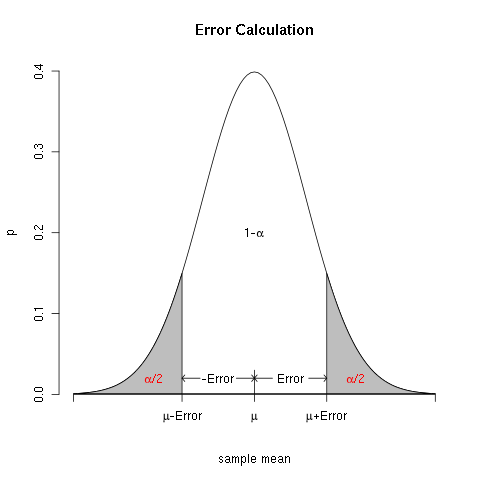
\includegraphics[width=4cm]{img/confidenceInterval}}

    \iftoggle{clicker}{%
      Clicker Quiz: \\
      \begin{tabular}{l@{\hspace{3em}}l@{\hspace{3em}}l@{\hspace{3em}}l}
        A: Yes  & B: No  & C: Maybe?
      \end{tabular}

    }

  }

  \vfill

\end{frame}


\begin{frame}
  \frametitle{The Problem}

  Situation: We think that the mean of $X$ is $\mu$ (some number).


  \begin{tabular}{ll}
    Problem: & $\bar{x}$ is a random variable. \\
    Problem: & $\bar{x}$ is our {\color{red}only way} of estimating $\mu$!
  \end{tabular}

\end{frame}

\begin{frame}{What do we do?}

  \begin{enumerate}
  \item<1-> We have some {\color{red}idea/belief} of what to expect.
  \item<2-> This is our {\color{red}hypothesis} of what we \textit{think} is happening.
  \item<3-> We want to {\color{red}make a case} for some change in how we interpret the
    situation.
  \item<4-> {\color{red}Assume} that the \textit{status quo} is good or better. (Call this the
    \textit{Null Hypothesis}, $H_0$.)
  \item<5-> {\color{red}Construct a hypothesis} about what we think is \textbf{think}
    is happening. (Call this the \textit{alternate hypothesis}, $H_a$.)
  \item<6-> Collect \textit{evidence} {\color{red}assuming $H_0$ is true}. 
  \item<7-> If the evidence is {\color{red}\textit{``highly unlikely''} under the
    assumed conditions} then reject the null hypothesis, otherwise we
    cannot reject the null hypothesis.
  \end{enumerate}
  
\end{frame}

\subsection{Examples}

\begin{frame}{Example}

  We think that interest rates for mortgages have decreased since last
  quarter.

  \vfill

  \only<2->
  {
    \begin{tabular}{l@{\hspace{2em}}l}
      $H_0$: & Interest rates are the same. \\
      $H_a$: & Interest rates have decreased.
    \end{tabular}
  }

  \vfill

  \only<3-> { Sample fifteen banks, find the mean change in interest
    rate, and ask if there is sufficient evidence to reject $H_0$.  }

  \vfill

\end{frame}

\begin{frame}{Example}

  We think that foreclosures have increased since last quarter.

  \vfill

  \only<2->
  {
    \begin{tabular}{l@{\hspace{2em}}l}
      $H_0$: & Foreclosure rates are the same. \\
      $H_a$: & Foreclosure rates have increased.
    \end{tabular}
  }

  \vfill

  \only<3->
  {
    Sample thirty properties at random, calculate a foreclosure rate, and ask if
    there is sufficient evidence to reject $H_0$.
  }

  \vfill

\end{frame}


\begin{frame}{Example}

  We think that a new commercial will change the demand for a product.

  \vfill

  \only<2->
  {
    \begin{tabular}{l@{\hspace{2em}}l}
      $H_0$: & The commercial has no impact. \\
      $H_a$: & The commercial has an impact.
    \end{tabular}
  }

  \vfill

  \only<3->
  {
    Play the commercial in ten markets. Monitor the sales in those markets, and ask if
    there is sufficient evidence to reject $H_0$.
  }

  \vfill

\end{frame}


\begin{frame}{Three Options!}

  In the proceeding examples there were three different options:
  \begin{itemize}
  \item Decrease,
  \item Increase,
  \item Change.
  \end{itemize}
  
\end{frame}


\begin{frame}{Example}

  We think that interest rates for mortgages have
  \textcolor{red}{\textbf{decreased}} since last quarter.

  \vfill

    \begin{tabular}{l@{\hspace{2em}}l}
      $H_0$: & Interest rates are the same. \\
      $H_a$: & Interest rates have \textcolor{red}{\textbf{decreased}}.
    \end{tabular}

  \vfill

    Sample fifteen banks, find the mean interest rate, and ask if
    there is sufficient evidence to reject $H_0$.

  \vfill

\end{frame}

\begin{frame}{Example}

  We think that foreclosures have \textcolor{red}{\textbf{increased}} since last quarter.

  \vfill

    \begin{tabular}{l@{\hspace{2em}}l}
      $H_0$: & Foreclosure rates are the same. \\
      $H_a$: & Foreclosure rates have \textcolor{red}{\textbf{increased}}.
    \end{tabular}

  \vfill

    Sample theory properties at random, calculate a foreclosure rate, and ask if
    there is sufficient evidence to reject $H_0$.

  \vfill

\end{frame}


\begin{frame}{Example}

  We think that a new commercial will \textcolor{red}{\textbf{change}} the demand for a product.

  \vfill

    \begin{tabular}{l@{\hspace{2em}}l}
      $H_0$: & The commercial has no impact. \\
      $H_a$: & The commercial has \textcolor{red}{\textbf{an impact}}.
    \end{tabular}

  \vfill

    Play the commercial in ten markets. Monitor the sales in those markets, and ask if
    there is sufficient evidence to reject $H_0$.

  \vfill

\end{frame}

\iftoggle{clicker}{%

  \begin{frame}{Clicker Quiz}

    I think that the mean stock price in a given sector has
    increased. I sample thirty stocks and determine the change in
    price for each one. What is the hypothesis test?

    \begin{tabular}{l@{\hspace{2em}}l} \hline
      A \\
      $H_0$: &  The mean price has not changed.\\
      $H_a$: & The mean price change is greater than zero. \\
      \\  \hline
      B \\
      $H_0$: &  The mean price has not changed. \\
      $H_a$: & The mean price change is less than zero. \\
      \\ \hline
      C \\
      $H_0$: &  The mean price has not changed.\\
      $H_a$: & The mean price change is not zero. \\ \hline
    \end{tabular}

    
  \end{frame}

}


\begin{frame}{Problem}

  \vfill

  $\bar{x}$ is a random variable.

  \vfill

  The data can \textbf{lie}!

  \vfill
  
\end{frame}


\begin{frame}{The Possibilities}

  \centerline{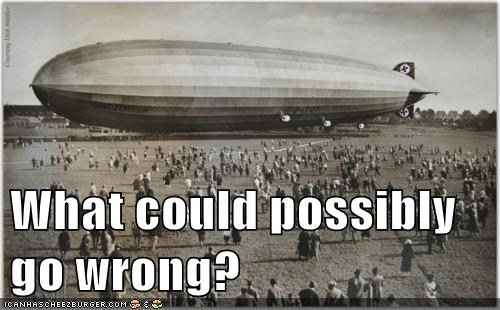
\includegraphics[width=3.0cm]{img/hindenburg}}

  \begin{eqnarray*}
    \mathrm{Data~-} & &
      \begin{array}{l@{\hspace{1em}}|c|c|} 
        \multicolumn{3}{r}{\mathrm{Reality}} \\ 
        \multicolumn{1}{c}{~} & \multicolumn{1}{c}{H_0
          \mathrm{~is~true}} & \multicolumn{1}{c}{H_0
          \mathrm{~is~false}} \\  
        \hhline{~--}
        \mathrm{Do~Not~Reject~}H_0 & 
\includegraphics[width=0.7cm]{img/smiley} & \mathrm{Type~II~Error} \\ \hhline{~|-|-|}
        \mathrm{Reject~}H_0 & \mathrm{Type~I~Error} & 
\includegraphics[width=0.7cm]{img/smiley} \\ \hhline{~--}
      \end{array}
  \end{eqnarray*}
  
\end{frame}


\begin{frame}{How To State Results}

  How you state your conclusions matter! It is an ethical issue in
  terms of conveying your assumptions and potential problems
  associated with the methodology.

  \begin{block}{Reject $H_0$}
    There is sufficient evidence to reject $H_0$ at the \#
    significance level assuming a normal distribution and a 
    standard deviation of \#.
  \end{block}

  \begin{block}{Cannot Reject $H_0$}
    There is not sufficient evidence to reject $H_0$ at the \#
    significance level assuming a normal distribution and a 
    standard deviation of \#.
  \end{block}

  
\end{frame}

\begin{frame}{The Methodology}

  What do we do?

  \begin{enumerate}
  \item Assume that $H_0$ is true.
  \item Ask, ``Are the data an unlikely result?''
  \end{enumerate}

  \only<2->
  {
    We want:
    \begin{itemize}
    \item The probability that we get our result to be ``small.''
    \item The probability that we get our result \textit{given our
        assumptions} is the significance level
      ($\alpha$). \textbf{\color{red} It is a conditional
        probability!}
    \end{itemize}
  }

  \only<3->
  {
    Note: We need to define this cut-off value, $\alpha$, \textbf{in
      advance!} i.e. before any data collection or manipulation.
  }
  
\end{frame}


\begin{frame}{Example}

  I see a publication that says that the mean house value in an area
  is \$215,000 with a standard deviation of \$35,000. I think that
  this is too high.

  \vfill

  \only<2->
  {

    \begin{tabular}{l@{\hspace{2em}}l}
      $H_0$: & The mean house price is \$215,000 or more. \\
      $H_a$: & The mean house price is \textcolor{red}{\textbf{less than \$215,000}}.
    \end{tabular}

    I will use a 5\% significance level.

  }

  \vfill

  \only<3->
  {

    Suppose that I take a random sample of ten homes and get a sample
    mean of \$198,000. Is the mean house price smaller than \$215,000?

  }

  \vfill

  
  
\end{frame}

% LocalWords:  Clarkson pausesection hideallsubsections
